\documentclass[border=10pt]{standalone}
\usepackage[UTF8]{ctex}
\usepackage{tikz}
\newcommand{\iwd}{1000}
\newcommand{\fs}[1]{\fontsize{#1 pt}{0pt}\selectfont}

\begin{document}
\begin{tikzpicture}[x=1pt, y=1pt]
\node at (0,0) {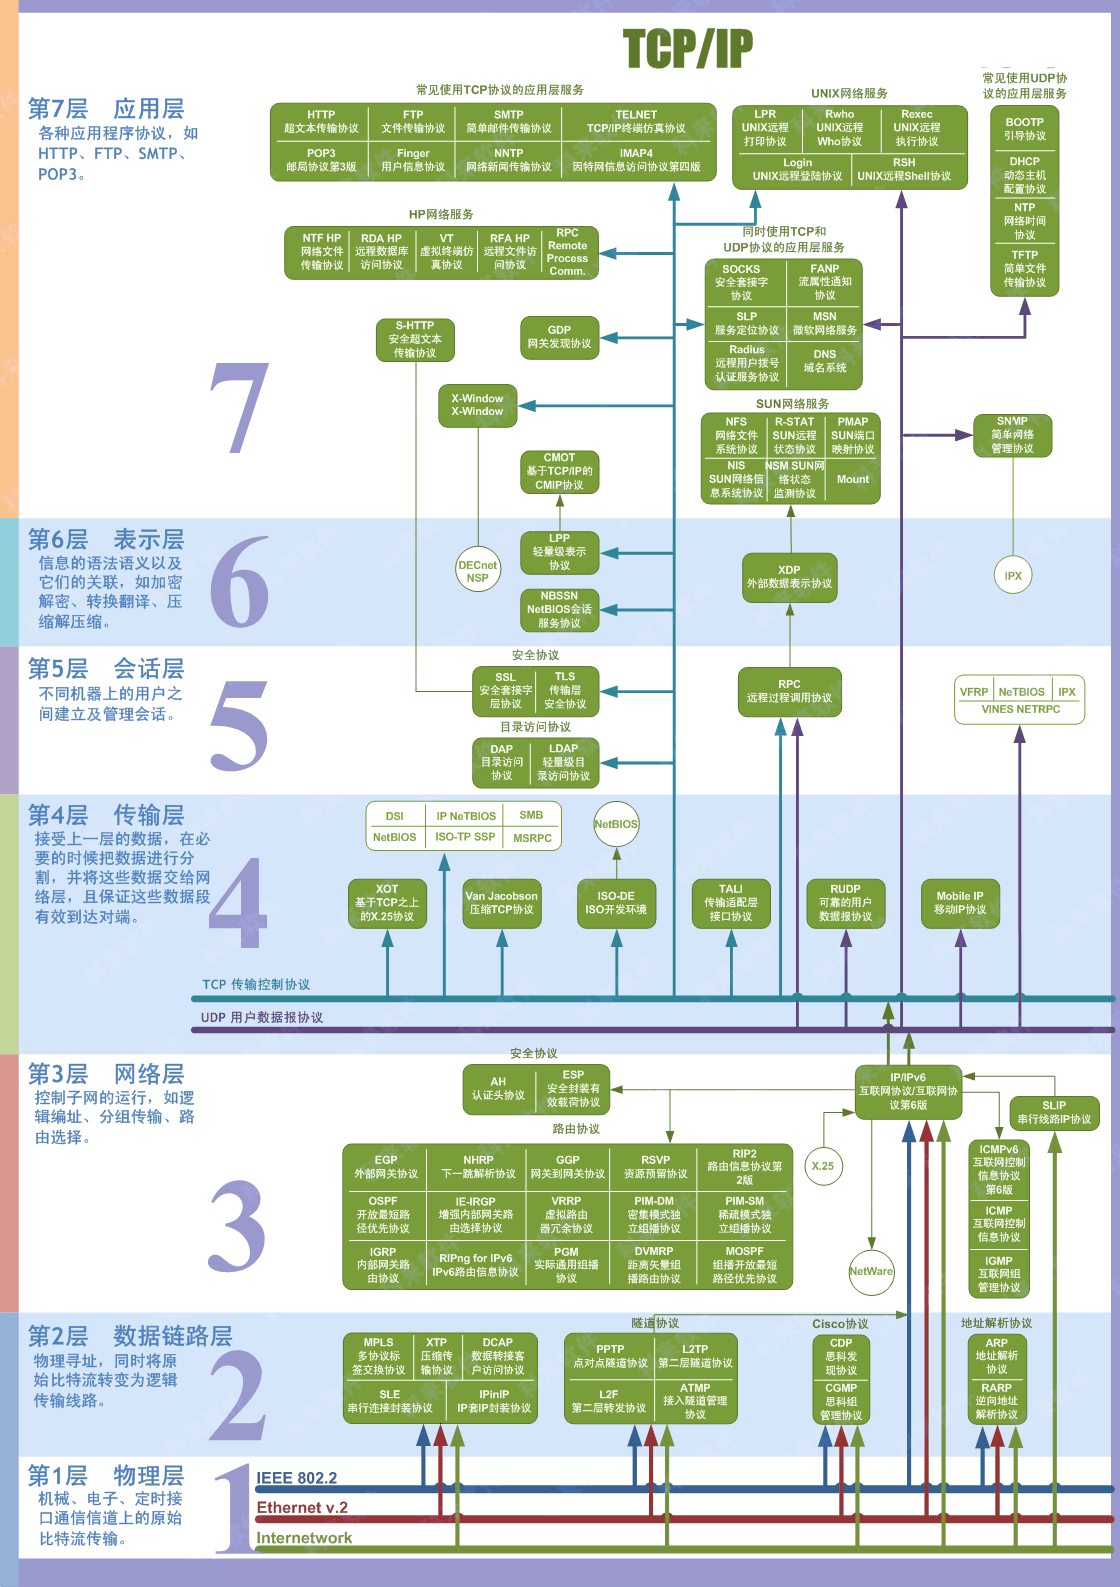
\includegraphics[width=\iwd pt]{tcp-ip.png}};
\draw[step=40pt, line width=0.5pt, opacity=0.7, black] (-\iwd/2, -\iwd/2*1.5) grid (\iwd/2, \iwd/2*1.5);
\fill [red] (0,0) circle (3pt);
% \node [draw=blue, font=\fs{20}] at (0,0) {你好};

\end{tikzpicture}
\end{document}